\chapter{Percusiones y choques}

\begin{miparrafo}
En algunas situaciones, como en los choques, se ejercen fuerzas muy intensas entre los sólidos durante un tiempo muy corto. 
Su efecto es un cambio súbito en la velocidad de los cuerpos, así como deformaciones (permanentes o no) y pérdida de energía en forma de calor o sonido. 
A estas fuerzas muy intensas ( $F = \infty$ ) que actúan en tiempos muy cortos ( $\Delta t \approx 0$) se les llama fuerzas impulsivas o de percusión.
En estos casos conviene utilizar el impulso de estas fuerzas por ser una cantidad $F \cdot \Delta t$ una cantidad finita.
Se llama percusión al impulso producido por una de estas fuerzas integrada al tiempo de actuación:
$\vec p =\displaystyle \int_{\Delta t}\vec F \dd t \approx \vec t \Delta t$

Características de las percusiones:

\begin{itemize}
\item $a=\dfrac F m = \infty \qquad$ aceleraciones muy altas
\item $\Delta v=a\Delta t=finito\qquad$ cambio infinito y súbito de velocidades
\item $\Delta s=v\Delta t=0\qquad $ posiciones congeladas
\end{itemize}

Cualquier situación en que se produzca un cambio brusco en la velocidades sin modificarse la posición se puede tratar como una percusión.
\end{miparrafo}

Fuerza media: $\displaystyle \quad \vec F_M=\dfrac 1 {\Delta t} \ \int_t^{t+\Delta t} 	\vec F \dd t$

Segunda de Newton: $\displaystyle \vec F=\dv{\vec p}{t} \to \int_{\vec p_1}^{\vec p_2} \dd \vec p = \int_t^{t+\Delta t} \vec F \dd t \to \vec p_2-\vec p_1=\vec F_M \Delta t$

Por definición, la percusión es:

$$\subrayado{\vec I_p = \displaystyle \int_t^{t+\Delta t} \vec F \dd t} \ ; \qquad \text{\emph{vector de percusión o impulso}}$$

Tenemos que $\quad \vec p_2=\vec p_1+ \vec I_p$. La percusión es una interacción que transcurre en un tiempo $\Delta t$ muy pequeño.

\section{Centro de percusión}

$\displaystyle \dv{\vec L}{t}=\vec M$.  Trabajaremos en sistema de referencia $CM$, así, $\vec M=\vec r\ ' \times \vec F$, con $\vec r\ '$ el vector de posición desde el $CM$ hasta el punto en que se aplica la $\vec F$ que da lugar a la percusión.

 $\vec p_2-\vec p_1=\Delta \vec p=\vec I_p =\vec F_M \Delta t \to \vec M_m=\vec r \ ' \times \dfrac{\Delta I_p}{\Delta t}$
 
 En valor medio: $\ \dfrac {\Delta \vec L}{\Delta t}=\vec M_m=\vec r\ ' \times \vec I_p \ \to \ \boldsymbol{\Delta \vec L = \vec r \ ' \times \vec I_p}$

Establecemos una \emph{restricción}: el cuerpo está ligado a un punto punto fijo del espacio de modo que el único efecto que producirá la percusión será la rotación del mismo.

$\Delta \vec L=I\Delta \vec \omega \ \to \ \Delta \vec \omega = \dfrac{\vec r\ ' \times \vec I_p}{I}$; ahora, $\vec r\ '$ es el vector que va desde el punto fijo que no gira hasta el punto que consideramos, en el que se produce la percusión.

Si $\vec r\ '=0$ el punto de percusión pasa exactamente por el punto que consideramos y $\Delta \vec \omega =\vec 0$. El cuerpo solamente girará si $\vec r\ '\neq 0$.

\emph{Llamaremos \textbf{centro de percusión} a aquel punto del sistema físico en el que hay que aplicar los impulsos para que los cojinetes o centros de rotación no vibren, que se resistan lo mínimo}. Esto es un problema técnico.

\begin{multicols}{2}
El impulso $\vec I_p$ ha de ser perpendicular a la recta que pasa por el punto fijo $O$ o centro de rotación, el centro de masas $CM$ y el centro de percusión $CP$. De no ser así, se podría descomponer en dos componentes, una de las cuales perjudicaría los cojinetes y dañaría el centro de rotación:

 $\ \vec I_p \ \bot \ \overrightarrow{O,CM}$
\begin{figure}[H]
	\centering
	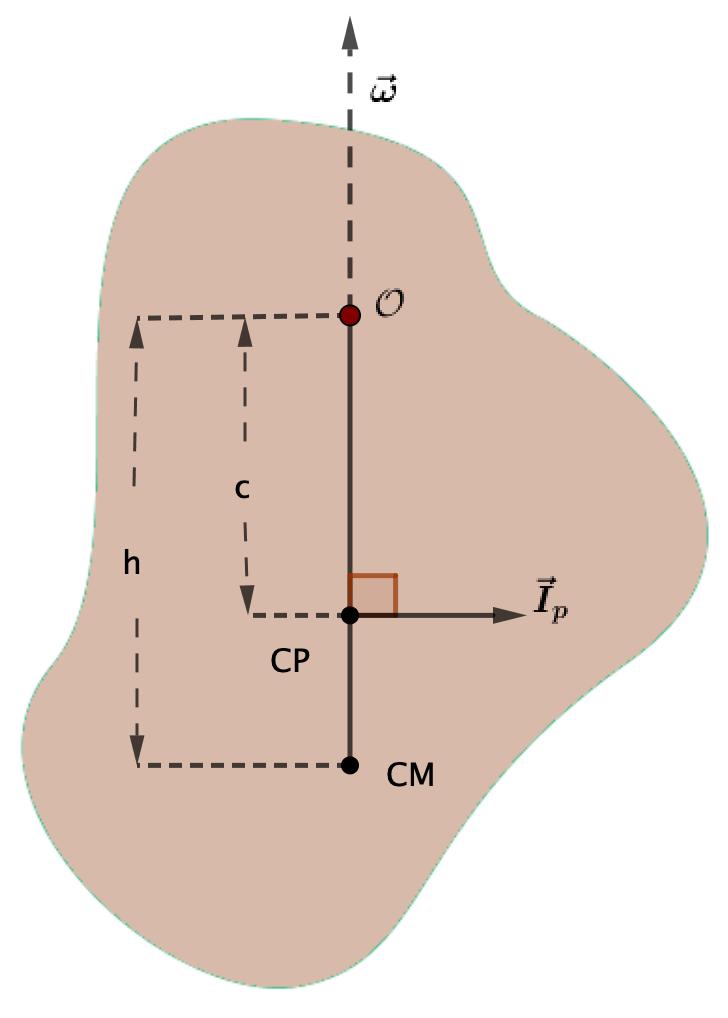
\includegraphics[width=.35\textwidth]{imagenes/imagenes17/T17IM01.png}
	\end{figure}	
\end{multicols}

$\vec p_2=\vec p_1+\vec I_p \ \to \ $ en general, $\quad \sum_i m_i\vec v_{2,i}= \sum_i m_i \vec v_{1,i} + \vec I_p$

Considerando la definición de centro de masas, $\ \vec R=\dfrac{\sum_i m_i \vec r_i}{\sum_i m_i}$, y derivando respecto al tiempo:
$\displaystyle \vec v_cm = \dfrac{\sum m_i \vec v_i}{m}; \quad \text{con} \ m=\sum_i m_i$, por lo que

$m\vec v_{CM,2}=m\vec v_{CM,1}+\vec I_p\to \vec I_p=m(\vec v_{CM,2}-\vec v_{CM,1})$, es decir, $\vec I_p=m\Delta \vec v_{CM}$ 


Por otra parte, $\ \vec v_{CM}=\vec \omega \times \vec h \to \Delta v_{CM}=h\Delta \omega \ \to \  I_p= m h \Delta \omega \quad (*)$ 

$\Delta \vec L = \vec r\ ' \times \vec I_p= I \vec \Delta \vec \omega$, y tenemos que $\vec r\ ' = \vec c \ \bot \ \vec I_p$, tendremos

$I \Delta \omega = c I_p \ \to \ (*) \quad \subrayado{\  \boldsymbol{c=\dfrac{I}{mh}} \ }$

\section{Colisiones o choques}

Vamos a efectuar un análisis de las colisiones o choques  desde un punto de vista microscópico. $\ b=$ parámetro de impacto.

Esta variación en la cantidad de movimiento se llama colisión o choque. Ocurre lo mismo con objetos macroscópicos, aunque no se observe bien

\begin{multicols}{2}
También puede ocurrir que una partícula incida sobre un blanco y salgan dos partículas distintas a la inicial. A este tipo de choques en los que se produce un intercambio en la naturaleza de las partículas entre su estado inicial y final se le llama \emph{choque inelástico}. Cuando las partículas l canal inicial son las mismas que las del canal final, se dice que el \emph{choque} es \emph{inelástico}. 
\begin{figure}[H]
	\centering
	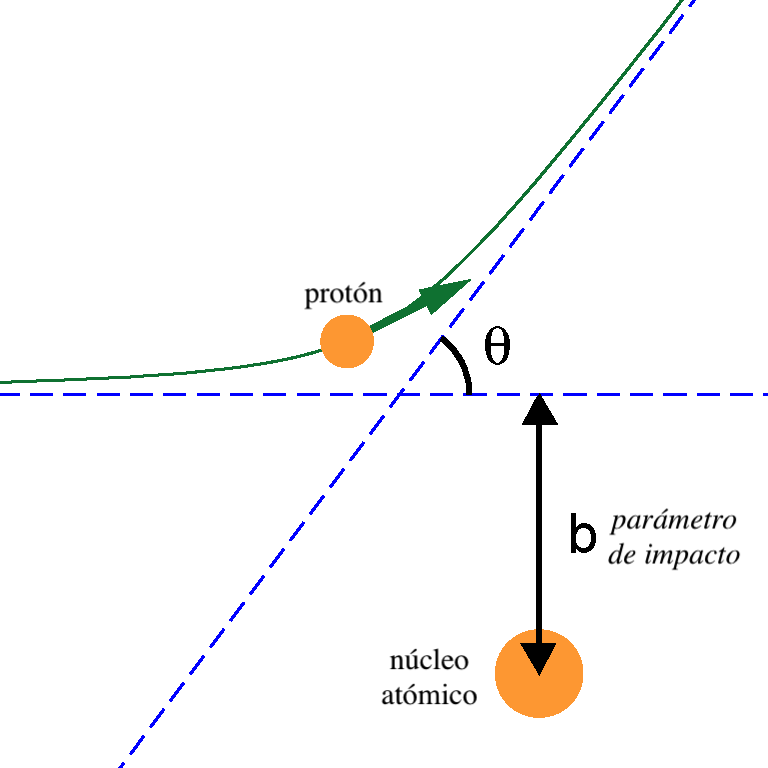
\includegraphics[width=.5\textwidth]{imagenes/imagenes17/T17IM02.png}
	\end{figure}
\end{multicols}

Un choque se caracteriza porque se tiene una partícula que se lanza sobre otra en un sistema aislado, ningún campo de fuerzas exteriores actúa sobre este sistema físico y la interacción solo se debe a las fuerzas interiores de las partículas que interactúan.

$2^a$ de Newton: $\ \displaystyle \dv{\vec p}{t}=\vec F^{(e)}=0 \ \Rightarrow \ \vec p=\overrightarrow{cte}$, la cantidad de movimiento total del sistema ha de conservarse.

$$\subrayado{ \ \vec p_1\ + \ \vec p_2 \ = \ \vec p_1\ '\ + \ \vec p_2\ ' \ }$$

Si no hay campo exterior, la $E$ mecánica total se conserva: la energía mecánica total en el canal de entrada ha de ser igual a la energía mecánica total en el canal de salida.

$$\subrayado{ \ \mathcal E_c \ + \ \mathcal E_{p12} \ = \ \mathcal E_c\ ' \ + \ \mathcal E_{p12}\ ' \ }$$

Introducimos ahora un parámetro que nos indicará la naturaleza de la interacción que va a tener lugar. 

Por definición se llama \emph{calor de reacción o balance energético}, $Q$, al valor:

\begin{equation}
\subrayado{\ Q\ =\ \mathcal E_c \ - \mathcal E_c\ ' \  = \ \mathcal E_{p12} \  - \ \mathcal E_{p12}\ '
\ }	
\end{equation}

$$\begin{cases}
\ \ \text{ si } \ \ Q>0 \ \to \ \mathcal E_c \ '>\mathcal E_c\  \quad \text{exotérmica} \\	
\ \ \text{ si } \ \ Q=0 \ \to \  \mathcal E_c\ '=\mathcal E_c \quad \\
\ \ \text{ si } \ \ Q<0 \ \to \ \mathcal E_c\ '<\mathcal E_c \quad \text{endotérmica} 
\end{cases}$$

Es conveniente utilizar el sistema centro de masas.

$\mathcal E_c \ '=\mathcal E_c + Q \ :\quad \dfrac 1 2 m_1 {v'}_{CM,1}^2 + \dfrac 1 2 m_2 {v'}_{CM,2}^2= \dfrac 1 2 m_1 v_{CM,1}^2 + \dfrac 1 2 m_1 v_{CM,2}^2+Q$

En el sistema $CM$, $\quad \vec P_T=0=\vec p_{CM,1}+\vec p_{CM,2}=\vec p\ '_{CM,1}+\vec p\ '_{CM,2}=\vec P\ '_T$

${p'}^2_{CM,1}={p'}^2_{CM,2}={P'}^2_{CM};\qquad {p}^2_{CM,1}={p}^2_{CM,2}={P}^2_{CM}$

$\dfrac 1 2 \dfrac{{p'}_{CM}^2}{m_1} +\dfrac 1 2 \dfrac{{p'}_{CM}^2}{m_2}=\dfrac 1 2 \dfrac{{p}_{CM}^2}{m_1}+\dfrac 1 2 \dfrac{{p}_{CM}^2}{m_2}+Q;\quad \dfrac 1 2 {{P'}^2_{CM}}\left( \dfrac 1 {m_1} + \dfrac 1 {m_2} \right) = \dfrac 1 2 {P^2_{CM}}\left( \dfrac 1 {m_1} + \dfrac 1 {m_2} \right)$

$\dfrac 1 {\mu_I}=\left( \dfrac 1 {m_1} + \dfrac 1 {m_2} \right) \text{ en el canal I};\ \ \ \dfrac 1 {\mu_{II}}=\left( \dfrac 1 {m_1} + \dfrac 1 {m_2} \right) \text{ en el canal II}$

\begin{equation} \subrayado{ \ 
\dfrac 1 2 \dfrac {{P'}_{CM}^2}{\mu_{II}} \ = \ \dfrac 1 2 \dfrac {{P}_{CM}^2}{\mu_{I}} \ + \ Q 	\ }
\end{equation}

En el canal de entrada, partícula incidente y blanco, se conoce $P_{CM}$, es un dato.  También $\mu$ (o $\mu_I\text{ y } \mu_{II}$) es un dato . En los choques elásticos se cumple $\mu_I=\mu_{II}$

Por ejemplo, un choque podría ser: $\ ^3He\ ( \ ^9Be\ , \ ^8 Be\ )\ \alpha$

También $\mu$ (o $\mu_I\text{ y } \mu_{II}$) es un dato.

Pasamos ahora a interpretar los choques macroscópicamente.

\section{Choque eslástico. Coeficiente de restitución.}

De nuevo, $2^a$ de Newton: $\ \displaystyle \dv{\vec p}{t}=\vec F^{(e)}=0 \ \Rightarrow \ \vec p=\overrightarrow{cte}$, la cantidad de movimiento total del sistema ha de conservarse.

$\vec I_p=\vec p_1\ ' - \vec p_1= -( \ \vec p_2 \ ' - \vec p_2 \ )$

\begin{figure}[H]
	\centering
	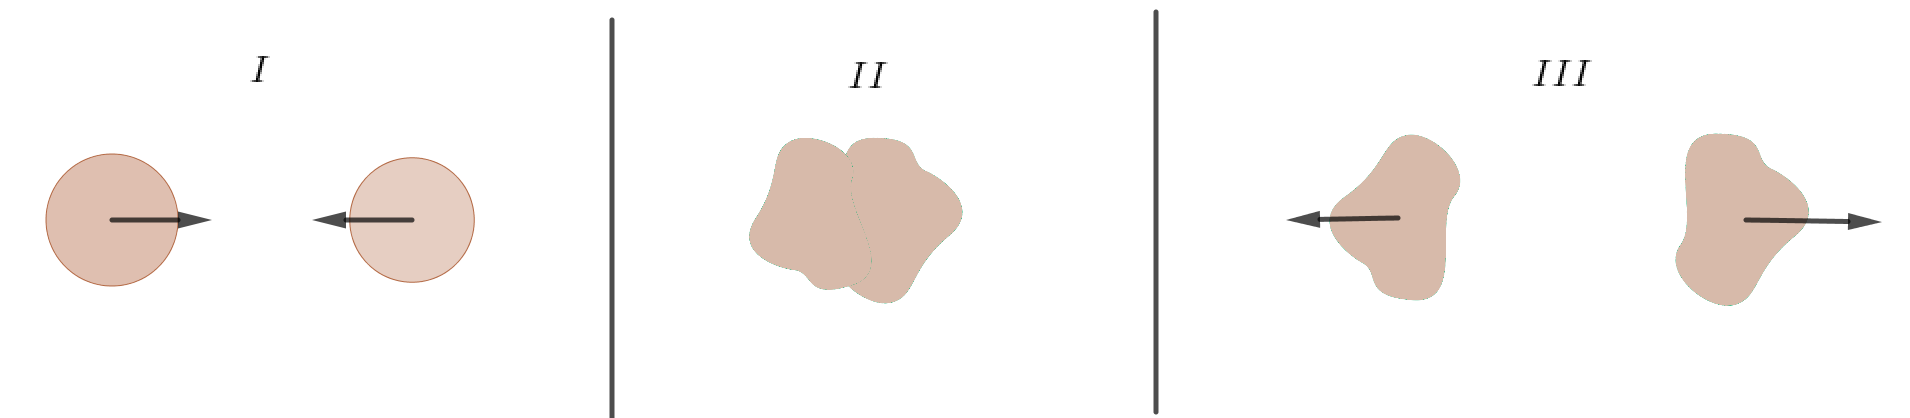
\includegraphics[width=1\textwidth]{imagenes/imagenes17/T17IM03.png}
	\end{figure}
	
	Se suele producir una deformación de los cuerpos tras el choque, la energía cinética inicial se invierte en energía cinética final más energía de deformación:  $\mathcal E_c=\mathcal E_c\ ' + Q$
	
Como $\vec p_{T}=cte \to \ \vec p_1+\vec p_2=\vec p_1\ ' + \vec p_2\ ' \ \to \ m_1\vec v_1+m2\vec v_2=m_1 \vec v_1\ ' + m_2 \vec v_2\ '$

Donde estamos suponiendo que los cuerpos que intervienen en la colisión conservas su masa, $Q$ solo representará la variación de la energía interna de los cuerpos que colisionan.

Generalmente, $\vec v_1$ y $\vec v_2$ son conocidas y nos preguntamos por los valores de $\vec v_1\ '$ y por $\vec v_2\ '$. Necesitamos una segunda ecuación vectorial (6 ecuaciones con 6 incógnitas.)

La segunda ecuación se introduce de forma empírica: \emph{Newton} define el \emph{\textbf{coeficiente de restitución}} como la \emph{proporción entre las velocidades relativas de los cuerpos antes y después de la colisión}. Es un coeficiente adimensional que solo depende de las propiedades elásticas de los cuerpos en colisión y se define como:

\begin{equation}
\subrayado{\ \boldsymbol{ \varepsilon = - \dfrac{v_2\ '-v_1\ '}{v_2-v_1}     } \ }	
\end{equation}

$\varepsilon \in [0,1]$. Según el valor de $\varepsilon$, los choques macroscópicos se clasifican en:

$$\begin{cases}
	\quad \varepsilon = 1 \quad \to \quad \text{choque elástico} \\
	\quad \varepsilon < 1 \quad \to \quad \text{choque parcialmente elástico} \\
	\quad \varepsilon = 0 \quad \to \quad \text{choque inelástico}
\end{cases}$$

\subsection[Choque central (particularización a una dimensión)]{Choque central (particularización a una dimensión)\subsectionmark{Choque central}}
\subsectionmark{Choque central}

$\varepsilon = 0 \to v_1\ '=v_2\ '$, los dos cuerpos salen juntos a la misma velocidad. Choque inelástico.

$varepsilon=1 \to v_2\ '-v_1\ '=v_2-v_1$, la energía cinética de salida es la misma que la de entrada, con lo que $\mathcal E_c=\mathcal E'_c+Q=0 \to Q=0$,  no hay deformación residual. Choque elástico.

El choque elástico es el que se suela dar a nivel microscópico. A nivel macroscópico, el choque elástico no se produce nunca.
En general ocurre que $0<\varepsilon<1$

\section{Estudio general del choque central.}

\emph{Choque central} es aquel que se produce según la línea que une los centro de masa de los cuerpos que interactúan. 
	
\begin{figure}[H]
	\centering
	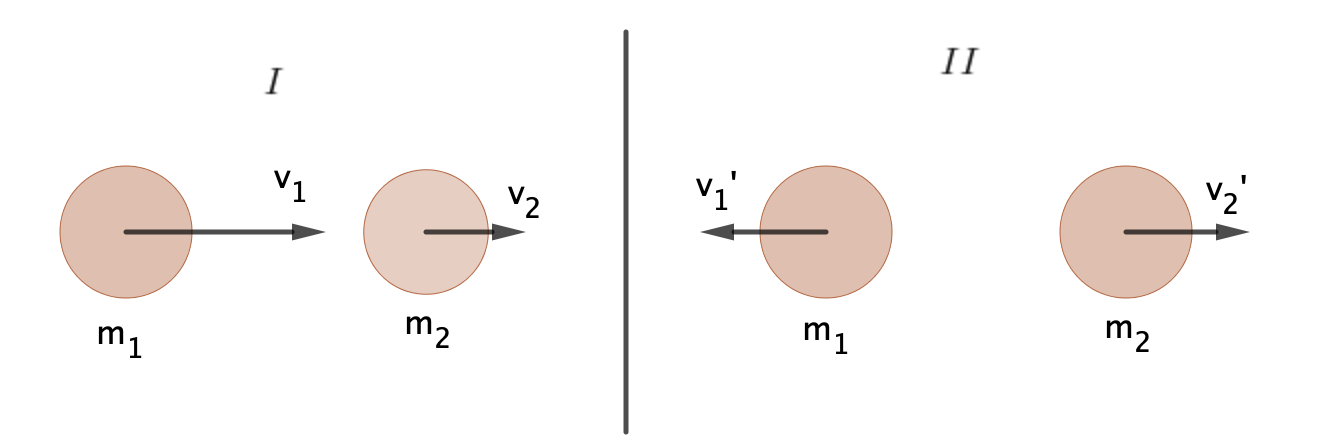
\includegraphics[width=1\textwidth]{imagenes/imagenes17/T17IM04.png}
	\end{figure}
	
Por convenio, escogemos como sentido positivo de las velocidades el que va hacia la derecha. Nuestros datos son $m_1, m_2, v_1, v_2, \varepsilon$ y nuestras incógnitas $v_1', v_2'$
	
Planteamos las ecuaciones:  $\ \ \begin{cases}
\ \ m_1v_1+m_2v_2=m_1v_1'+m_2v_2' \\ \ \ \varepsilon (v_2-v_1)=-v_2'+v_1'	
\end{cases}$

Despejando, por la regla de Cramer, se obtiene:

\begin{eqnarray} 
\label{velocidades-choques}
	 \boldsymbol{\subrayado{v_1'=\dfrac{m_1-\varepsilon m_2}{m_1+m_2}v_1 + \dfrac {(1+\varepsilon)m_2}{m_1+m_2}v_2}} \nonumber \\
	\boldsymbol{\subrayado{v_2' = \dfrac{(1+\varepsilon)m_1}{m_1+m_2}v_1 + \dfrac{m_2-\varepsilon m_1}{m_1+m_2}v_2}} 
\end{eqnarray}

Se observa que si $\varepsilon = 0$, choque inelástico, $v_1'=v_2'=\dfrac{m_1v_1+m_2v_2}{m_1+m_2}$, los dos cuerpos salen empotrados como un solo cuerpo después del choque con una velocidad igual a la de su $CM$, como era de esperar.

La percusión, $\vec I_p$, es máxima para choques elásticos, $\varepsilon=1$. La percusión es mínima para choques inelásticos, $\varepsilon=0$.

En los choques, al balance energético o calor de reacción $Q$ se le suele llamar $D$, \emph{\textbf{efecto destructor}}: $\mathcal E_c=\mathcal E'_c+Q \leftrightarrow \mathcal E_c=\mathcal E'_c+D;\quad Q=D$
	
El efecto destructor $D$ se puede expresar en función del coeficiente de restitución $\varepsilon$.

$D=\mathcal E_c-\mathcal E'_c=\Delta  \mathcal E_c=	\dfrac{(1-\varepsilon)^2m_1m_2}{2m_1m_2}(v_1-v_2)^2$

$D$ depende del cuadrado de la velocidad relativa, $v_1-v_2$.

En el choque elástico, $\varepsilon = 1 \to Q=0 \to D=0$. El valor máximo de $D$ se obtiene para $\varepsilon=0$, en el choque inelástico.

$D_{max}=	\dfrac{m_1m_2}{2m_1m_2}(v_1-v_2)^2=\dfrac 1 2 \mu v^2$, con $\mu$ la masa relativa y $v$ la velocidad del $CM$, es la energía cinética en $CM$.
	
Es interesante definir el \emph{\textbf{coeficiente de restitución de energía}} ,$\eta$ así:

$$\boldsymbol{\eta=\dfrac {\mathcal E'_c}{\mathcal E_c}}; \qquad \boldsymbol{ D}=\mathcal E_c-\mathcal E'_c=\left(1-\dfrac{\mathcal E'_c}{\mathcal E_c}\right) \mathcal E_c=\boldsymbol{ (1-\eta)\mathcal E_c}$$


$$\begin{cases}
	\quad \eta = 1 \quad \to \quad \text{choque elástico} \\
	\quad \eta < 1 \quad \to \quad \text{choque parcialmente elástico} \\
	\quad \eta = 0 \quad \to \quad \text{choque inelástico}
\end{cases}$$	

\section{Casos particulares de los choques centrales}

\vspace{10mm} %***********************************************
\subsection{Choque de dos cuerpos de igual masa}

$$m_1=m_2 \quad \to \quad 
\begin{cases}
\ v'_1\ =\ \dfrac{1-\varepsilon}{2} \ v_1 \ +\  \dfrac{1+\varepsilon}{2} \ v_2 \\	
\ v'_2\ =\ \dfrac{1+\varepsilon}{2} \ v_1\ +\  \dfrac{1-\varepsilon}{2} \ v_2 
\end{cases}$$

Choque elástico, $\varepsilon=1 \ \to \ v'_1=v_2 \ \wedge \ v'_2=v_1$. Si las bolas son del mismo color, parecerá que no hubiese habido choque.

Choque inelástico: $\varepsilon=0 \to \ v'=\dfrac{v_1+v_2}{2}=v_{CM}$


\vspace{10mm} %***********************************************
\subsection{Choque contra un cuerpo que está en reposo cuya masa es muy grande}


$$m_1<<m_2;\ v_2=0 \ \to \ \textcolor{gris}{\left( \dfrac{m_1}{m_2}\to 0 \right)} \ \to \ \begin{cases}
 \ \ v'_1\ =\ -\varepsilon \ v_1 \\ \ \  v'_2=0	
\end{cases}$$
\textcolor{gris}{ Hemos dividido las ecuaciones (\ref{velocidades-choques}) por $m_2$}

Este es el caso de una bola que se deja caer sobre el suelo desde cierta altura.

El cuerpo de masa grande no se mueva y el de masa pequeña \emph{rebota} (signo contrario de la velocidad). $v'_1 \leq v_1$, el cuerpo rebota con velocidad menor o igual a con la que incide. 

Ahora, el coeficiente de restitución es:

\begin{multicols}{2}
$\eta = \dfrac{\mathcal E'_c}{\mathcal E_c}=\dfrac{mgh'}{mgh} \to \eta=\dfrac{h'}{h};$

$\varepsilon=-\dfrac{v'_1}{v_1}\to$

$ \varepsilon^2=\dfrac{{v'_1}^2}{{v_1}^2}=\eta \to $

$\varepsilon =\sqrt{\eta}=\sqrt{\dfrac{h'}{h}}$	
\begin{figure}[H]
	\centering
	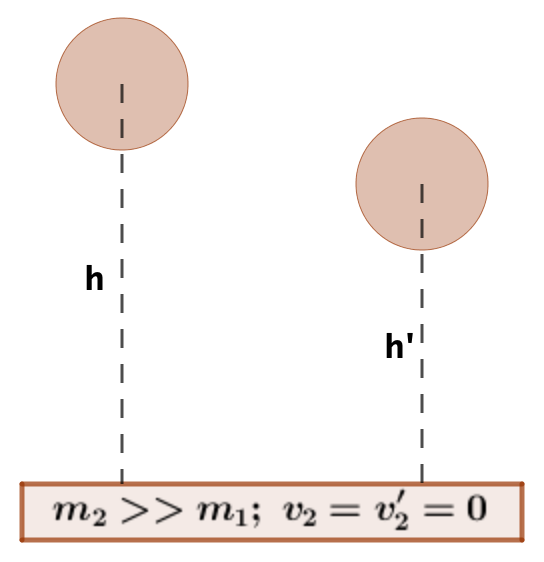
\includegraphics[width=.35\textwidth]{imagenes/imagenes17/T17IM05.png}
	\end{figure}	
\end{multicols}
	
Choque elástico, $\varepsilon=1 \to $ el cuerpo rebota.

Choque inelástico, $\varepsilon=0 \to $ el cuerpo se queda pegado al suelo.

\subsection{Choque de un cuerpo contra otro muy masivo que se dirige hacia él}


$$m_1>>m_2;\ v_2=0\ \to \ \textcolor{gris}{\left( \dfrac{m_2}{m_1}\to 0 \right)} \ \to \ \begin{cases}
 \ \ v'_1\ = v_1 \\ \ \  v'_2=(1+\varepsilon)\ v_1	
\end{cases}$$

\textcolor{gris}{ Hemos dividido las ecuaciones (\ref{velocidades-choques}) por $m_1$}

Este es el caso de un mosquito chocando contra una locomotora.

El cuerpo super masivo ni se entera, sale del choque con la misma velocidad. El cuerpo poco masivo sale con una velocidad mayor a la que tenía.

Choque elástico, $\varepsilon=1$, el cuerpo poco masico sale con velocidad doble.

Choque elástico, $\varepsilon=0$, los cuerpos salen pegados con la velocidad del cuerpo supermasivo.

Ahora, el efecto destructor es:

$D=\dfrac{(1-\varepsilon^2)m_1m_2}{2(m_1+m_2)} (v_1-v_2)^2=\dfrac 1 2 (1-\varepsilon^2)m_2v_1^2$ 

Si $\varepsilon=0$, choque inelástico (mosquito-locomotora), $v'_2=(1+\varepsilon)v_1=v_1$ y tenemos que $D=\dfrac 1 2 m_2 v_1^2$,  que coincide con la energía cinética que adquiere el cuerpo atropellado. La destrucción alcanza el máximo.

En el caso anterior, el efecto destructor recae sobre el cuerpo que incide.

\section{Choque oblícuo}

\begin{multicols}{2}
$\quad$

Tiene lugar cuando incide un cuerpo de masa pequeña contra una pared reflectora (masa mucho mayor y en reposo), existiendo un ángulo de incidencia y uno de reflexión respecto de la dirección normal a la pared. 
\begin{figure}[H]
	\centering
	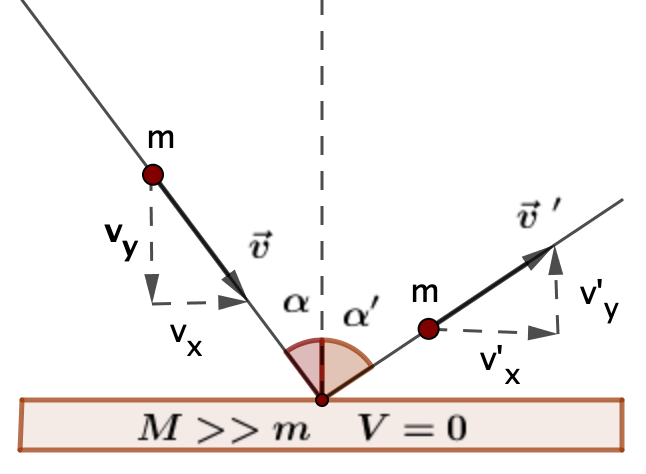
\includegraphics[width=.5\textwidth]{imagenes/imagenes17/T17IM06.png}
	\end{figure}
\end{multicols}

La componente $x$ de la cantidad de movimiento se conserva: $v_x=v\sin \alpha =v'_x$. Para la componente $y$ es como el caso del cuerpo que cae verticalmente, ale rebotado (signo menos) $v'_y=-\varepsilon v_y=-\varepsilon v \cos \alpha$

$\tan \alpha' =\dfrac {v'_y}{v'_x}=\dfrac{v \sin \alpha}{\varepsilon v \cos \alpha}=\dfrac 1 \varepsilon \tan \alpha$, se tiene que:

\begin{equation}
\boldsymbol{ \tan \alpha' \ =\ \dfrac 1 \varepsilon \ \tan \alpha }
\end{equation}

Solo se cumple la ley óptica de la reflexión en los casos en que $\varepsilon =1$, en los choques elásticos, $\tan \alpha' =  \tan \alpha \to \alpha=\alpha'$

En general, $\ \boldsymbol{\alpha \ \geq \ \alpha' \ }$

Choque inelástico: $\varepsilon = 0 \to \tan \alpha'=\infty \to \alpha'=90^o$, el cuerpo que impacta no rebota, se desliza por el suelo.

\section{Problemas}

\begin{prob}
Una varilla de longitud $L$ y masa $M$ puede girar libremente alrededor de un pivote situado en un extremo $A$ de la misma. Una bala de masa $m$ y velocidad $v$ golpea la varilla a una distancia $\boldsymbol{a}$ de $A$ y se incrusta en ella.

Encontrar en momento angular respecto a a $A$ y la cantidad de movimiento inmediatamente antes y después del choque. ?`Cuál es la $Q$ de la colisión?	
\end{prob}

\begin{multicols}{2}
--- Momento angular.

inmediatamente antes l choque: 

$L=mav$

Como $\displaystyle \dv{\vec L}{t}=\vec M^{(e)}=0$, por ser $\vec F\ || \ \vec r$, entonces $\vec L=cte$, por lo que inmediatamente después: 

$L=mav$

--- Cantidad de movimiento:
\begin{figure}[H]
	\centering
	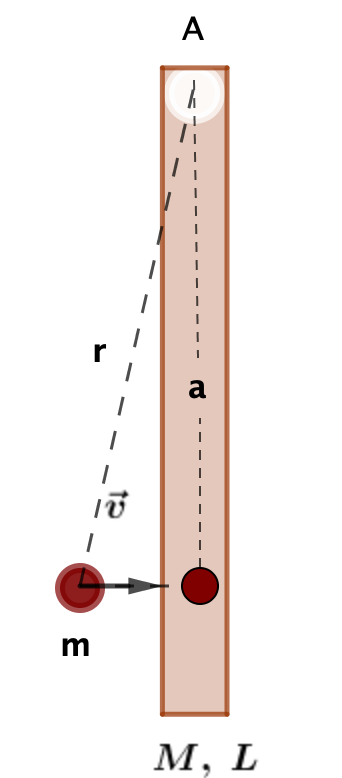
\includegraphics[width=.2\textwidth]{imagenes/imagenes17/T17IM08.png}
	\end{figure}
\end{multicols}
inmediatamente antes del choque: $\quad p=mv$

después el choque: $\quad p=p_{bala}+p_{barra}$, ambas giran con $\omega$

$p_{bala}=mv_{\text{después}}=m a\omega$

$p_{barra}=\displaystyle \int_L \dd p=\int_L v\dd m=\int_0^L \omega x \dd m =\int_0^L \omega x \rho \dd x=  \omega \rho \int_0^L x \dd x= \omega \rho \dfrac {L^2}{2}=\omega \dfrac {M}{L} \dfrac{L^2}{2}=\dfrac 1 2 \omega M L$

Luego, $\quad p=p_{bala}+p_{barra}=\omega \left( ma + \dfrac 1 2 ML \right)$

Del resultado anterior del momento angular,

 $L_{\text{antes}}=L_{\text{después}} \to mav=I\omega \to \omega=\dfrac{mva}{I}=\dfrac{mva}{\dfrac 1 3 ML^2+ma^2} $

por lo que, $p_{\text{después}}=\dfrac{mva}{\dfrac 1 3 ML^2+ma^2}\left( ma + \dfrac 1 2 ML \right) = mv\left( \dfrac{1+\dfrac{ML}{2ma}}{1+\dfrac{ML^2}{3ma^2}} \right)$

--- Vamos a por el balance energético: 

$\mathcal E_c=\mathcal E'_c+Q \to Q=\mathcal E_c-\mathcal E'_c=\dfrac 1 2 m v^2 - \dfrac 1 2 I \omega^2 = \dfrac 1 2 m v^2 - \dfrac 1 2 I \dfrac{L^2}{I^2}= \dfrac 1 2 \left( mv^2 - \dfrac{m^2v^2a^2}{\dfrac 1 3 ML^2+ma^2} \right)$

\begin{prob}
Se pone a girar un cazo hemiesférico de radio $a$ alrededor de su eje vertical con velocidad angular $\omega$. Si se coloca una canica de masa $m$ en el cazo giratorio, después de algún tiempo se queda a una distancia $d$ del eje. Encontrar $d$ en función de $\omega$.	
\end{prob}
\begin{multicols}{2}
$mg\sin \theta=F_c \cos \theta$

$\tan \theta=\dfrac{F_c}{mg}=\dfrac{m\dfrac{v^2}{d}}{mg}=\dfrac{\omega^2 d}{g}$

\textcolor{gris}{$(v=\omega d)$}

Geométricamente: 

$\tan \theta=\dfrac{d}{\sqrt{a^2-d^2}}$

Luego $d=\sqrt{a^2-\dfrac{a^2}{g^4}}$
\begin{figure}[H]
	\centering
	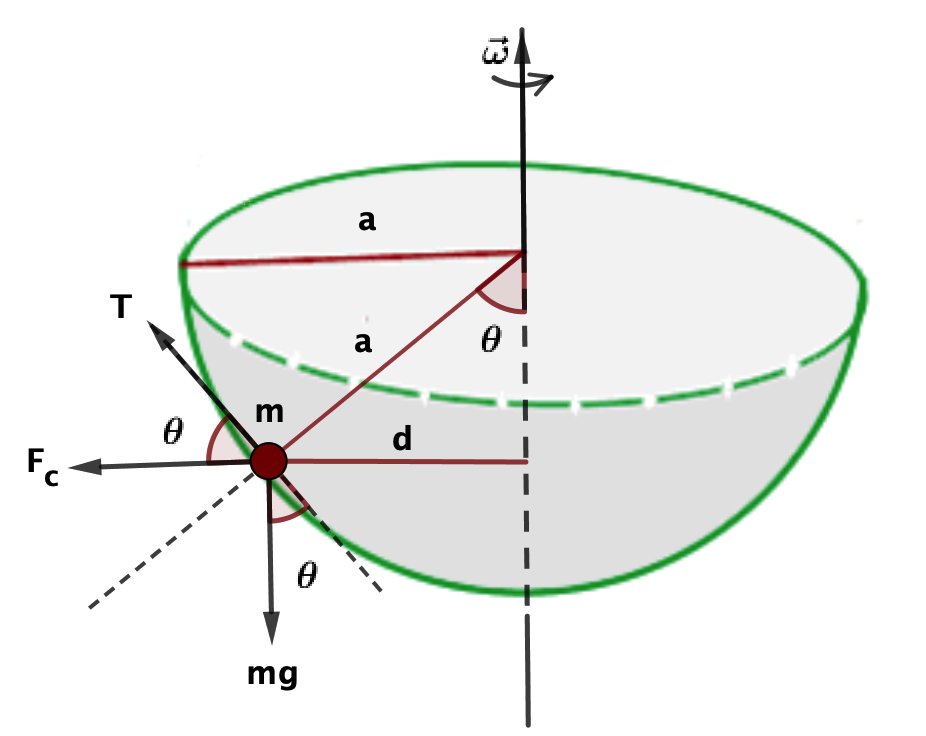
\includegraphics[width=.55\textwidth]{imagenes/imagenes17/T17IM10.png}
	\end{figure}
\end{multicols}

\vspace{5mm} %****************************************************
\begin{prob}
	Un disco uniforme de masa $M$ y radio $R$ gira alrededor de un eje horizontal que pasa por su centro con velocidad angular $\omega$. En un momento determinado, una astilla de masa $m$ se desprende del borde del disco, de modo que la astilla sube verticalmente sobre el punto en que se desprendió. ?`Qué altura alcanzará la astilla?, ?`cuál será la velocidad angular del discos después del desprendimiento?.
\end{prob}

\begin{multicols}{2}
--- altura alcanzada:

$h=v_1t-\dfrac 1 2 g t^2$

$v_f=v_1-gt=0$

$h=\dfrac 1 2 \dfrac{v_1^2}{g}=\dfrac 1 2 \dfrac{\omega_1^2 R}{g}$

--- velocidad angular final:

$I\omega=I_f \omega_f$

$\omega_f=\omega\  \dfrac{\dfrac 1 2 MR^2}{\dfrac 1 2 (M-m)R^2}=\omega \  \dfrac{M}{M-m}$

Si $M>>m \to \omega_f \approx \omega$
\begin{figure}[H]
	\centering
	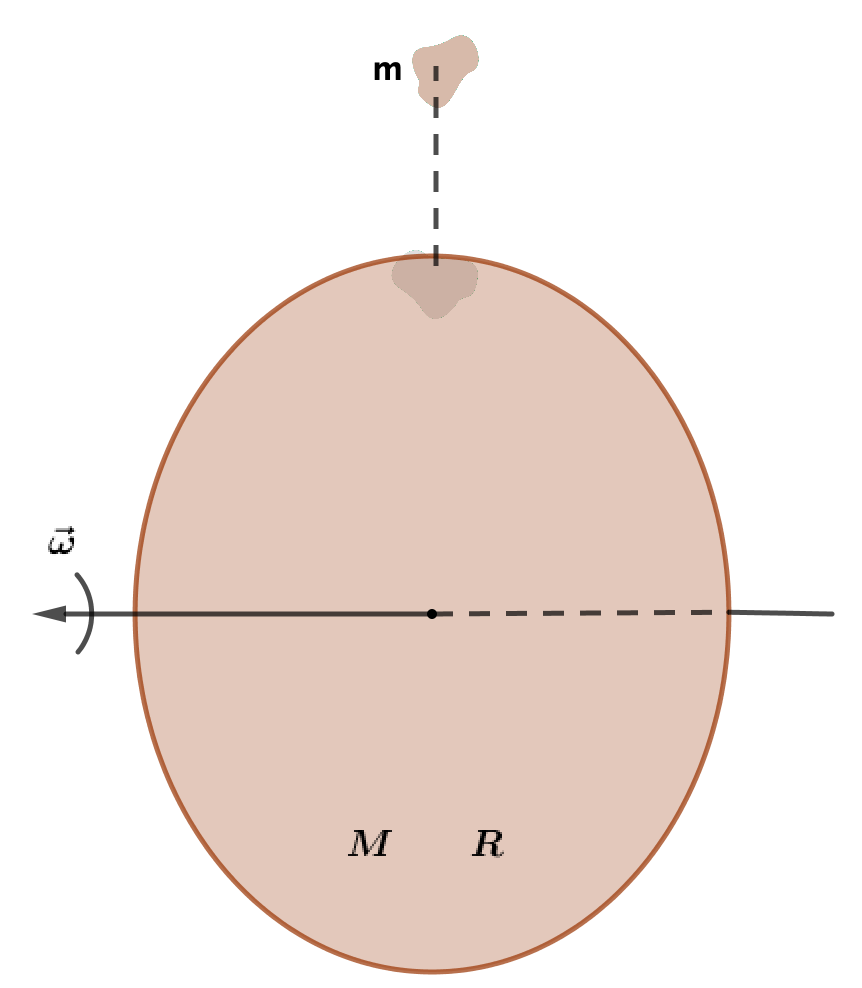
\includegraphics[width=.55\textwidth]{imagenes/imagenes17/T17IM11.png}
	\end{figure}	
\end{multicols}

\begin{prob}
Una granada en reposo en sistema laboratorio, estalla en dos fragmentos. Encontrar las energías cinéticas de los fragmentos en función de $Q$.	
\end{prob}

Puesto que se conserva el momento angular y la granada estaba inicialmente en reposo:
$\vec p=0=\vec p_1+\vec p_2$, en módulo, $p_1=p_2$

$Q=\mathcal E'_c-\mathcal E_c=\dfrac{p_1^2}{2m_1}+\dfrac{p_2^2}{2m_2}-0$, como $p_1=p_2$, 

tenemos que : $Q=\dfrac 1 2 \left( \dfrac 1 {m_1}+\dfrac 1{m_2} \right)p_1^2$

De aquí, $\ p_1=p_2=\sqrt{2\mu Q}$, por lo que 

$\mathcal E_{c,1}=\dfrac{p_1^2}{2m_1}=\dfrac{m_2Q}{m_1+m_2}; \qquad \mathcal E_{c,2}=\dfrac{p_2^2}{2m_2}=\dfrac{m_1Q}{m_1+m_2}$


\vspace{5mm} %****************************************************
\begin{prob}
Analizar el movimiento de una pelota que se deja caer desde cierta altura $h$ contra el suelo, siendo $\epsilon$ su coeficiente de restitución.	
\end{prob}

\begin{multicols}{2}
$v'_x=v_x; \quad v'y=-\varepsilon v_y$

Suponemos un tiro vertical $v_x=0; \ v_y=0$

------ \underline{alturas en los rebotes}:

--- Primer rebote:

$mgh=\dfrac 1 2 m v^2 \to v=\sqrt{2gh}$

después el choque: $v'=\varepsilon v$

asciende hasta 
\begin{figure}[H]
	\centering
	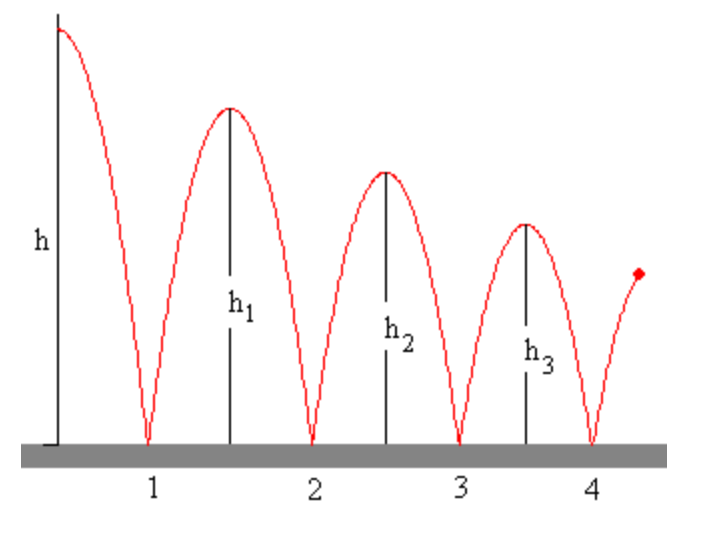
\includegraphics[width=.55\textwidth]{imagenes/imagenes17/T17IM12.png}
	\end{figure}	
\end{multicols}
$h_1: \quad \dfrac 1 2 m {v'}^2=mgh_1 \to h_1=\varepsilon^2 h$

--- segundo rebote: $\ \dfrac 1 2 m v''^2=mgh_1 \to v''=\sqrt{2gh_1}$

después del choque $\ v'''=\varepsilon v''$

asciende hasta $\ h_2:\quad \dfrac 1 2 m {v'''}^2=mgh_2 \to h_2=\varepsilon^2 h_1=\varepsilon^4 h$

--- rebote enésimo: $\ h_n=\varepsilon^{2n} h$

\textcolor{gris}{Suma de los infinitos términos de una PG de $r<1:\quad S_{\infty}=\dfrac{a_1}{1-r}$.}

La suma de todas las alturas, distancia en el eje $Y$ que recorre la pelota hasta detenerse, será:

$h_{total}=h(1+\varepsilon^2+\varepsilon^4+\cdots +\varepsilon^{2n}+\cdots )=\dfrac {h}{1-\varepsilon^2}$

\textbf{análisis de casos extremos:}

\begin{itemize}
\item Choque elástico: $\ \varepsilon=1 \to h_{total}\to \infty$, la pelota no cesa de rebotar.
\item Choque inelástico: $\ \varepsilon=0\to h_{total}=h$, la pelota cae al suelo y se queda pegada a él.	
\end{itemize}

------ \underline{Pérdida de energía}:

$\Delta E_1=\dfrac 1 2 m (v'^2-v^2)=(\varepsilon^2-1)mgh$

$\Delta E_2=\dfrac 1 2 m (v''^2-v'^2)=(\varepsilon^2-1)mgh_1= \varepsilon^2(\varepsilon^2-1)mgh$

$\Delta E_n=(\varepsilon^2-1)mgh_{n-1}=\varepsilon^{2(n-1)}(\varepsilon^2-1)mgh$

$\Delta E=\Delta E_1+\Delta E_2+ \cdots + \Delta E_n+\cdots =mgh(\varepsilon^2-1)(1+\varepsilon^2+\cdots + )=mgh\dfrac{\varepsilon^2-1}{1-\varepsilon^2}=-mgh.\quad $Como era de esperar.

------ \underline{Tiempo hasta detenerse}:

$h=\dfrac 1 2 gt_0^2 \to t_0=\sqrt{\dfrac {2h}{g}}$

$t_1=2 \sqrt{\dfrac{2h_1}{g}}=2\sqrt{\dfrac{2\varepsilon^2 h}{g}}=2\varepsilon t_0$

$t_2=2\sqrt{\dfrac{2h_2}{g}}=2\sqrt{\dfrac{2\varepsilon^4h}{g}}=2\varepsilon^2 t_0$

$t_n=2\varepsilon^n t_0$

$t=t_0+t_1+t_2+ \cdots + t_n+\cdots =t_0+t_0(\varepsilon+\varepsilon^2+\cdots )=t_0+t_0 \dfrac{\varepsilon}{1-\varepsilon}$

$t=t_0\dfrac{1+\varepsilon}{1-\varepsilon}=\dfrac{1+\varepsilon}{1-\varepsilon} \sqrt{\dfrac{2h}{g}}$

------ Si \underline{la pelota se lanza horizontalmente} con velocidad $v_x$, la distancia recorrida en el eje x hasta detenerse en sus rebotes es:

$x=v_x t=v_x \dfrac{1+\varepsilon}{1-\varepsilon} \sqrt{\dfrac{2h}{g}}$




\newpage %********************************************
\begin{myblock}{El péndulo balístico}

El péndulo balístico es un dispositivo que permite determinar la velocidad de un proyectil.

\begin{multicols}{2}
\vspace{2mm} Este péndulo está constituido por un bloque grande de madera, de masa $M$, suspendido mediante un hilo vertical, como se ilustra en la figura. El proyectil, de masa $m$, cuya velocidad $v$ se quiere determinar, se dispara horizontalmente de modo que choque y quede incrustado en el bloque de madera.
\begin{figure}[H]
	\centering
	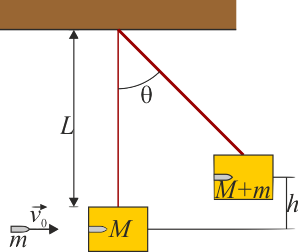
\includegraphics[width=.5\textwidth]{imagenes/imagenes17/T17IM07.png}
	\end{figure}
\end{multicols}
\vspace{2mm} Si el tiempo que emplea el proyectil en quedar detenido en el interior del bloque de madera es pequeño en comparación con el período de oscilación del péndulo, el hilo de suspensión permanecerá casi vertical durante la colisión (bastará con que el hilo sea suficientemente largo). 

\vspace{2mm} Supongamos que el centro de masa del bloque asciende a una altura $h$ después de la colisión. Entonces, conocidos las masas del proyectil y del bloque y el ascenso de este después del choque, la velocidad del proyectil viene dada por 

$$v=\left( 1 + \dfrac M m \right) \sqrt{2gh}$$

\vspace{2mm} Ecuación que se obtiene de aplicar la conservación del momento lineal, $mv=(M+m)V$ y la conservación de la energía mecánica $\dfrac 1 2 (M+m) V^2=(M+m)gh$.
\end{myblock}


